\documentclass{article}
\title{CSCI 2200 HW1}
\author{Xinshi,Wang}
\usepackage[letterpaper,textwidth=5.5in,right=0.6in,textheight=9in,left=0.6in,top=0.7in,bottom=0.7in]{geometry}
\usepackage{scrextend}
\usepackage{graphicx}
\usepackage{xcolor}
\usepackage{amssymb}
\usepackage{amsmath}
\usepackage{setspace}
\usepackage{mathrsfs}
\usepackage[utf8]{inputenc}
\usepackage{mathtools}
\begin{document}
\noindent
CSCI 2200 HW3\\
Wang Xinshi\\

%Q 12.8 starts from here
\begin{addmargin}[2em]{2em}
	\text{\bf Problem 15.15} Among 400 students, 150 are in math, 120 are in bio and 50 are math-bio duals. What are the chances a random student is in: (a) math or bio (b) bio and not math (c) neither math nor bio?\\
	
	\noindent (a)$\left |Math \cup Bio \right| = \left |Math \right| + \left |Bio \right| - \left |Math \cap Bio \right|$.

	Thus
	\begin{align*}
		P(\left |Math \cup Bio \right|) &= P(\left |Math \right|) + P(\left |Bio \right|) - P(\left |Math \cap Bio \right|)\\
		&= \dfrac{150}{400}+\dfrac{120}{400}-\dfrac{50}{400}\\
		&= \dfrac{11}{20}
	\end{align*} 

	\noindent (b)$\left |Math^c \cap Bio-Math \right| = \left |Bio-Bio \ capMath \right|$, since biology is a subset of not math.
		
	Thus
	\begin{align*}
		P(\left |Math^c \cap Bio \right|) &= P(\left |Bio - Bio \cap Math \right|)\\
		&= \dfrac{70}{400}\\
		&= \dfrac{7}{40}
	\end{align*} 

	\noindent (c)$\left |Math \cup Bio \right|^c = \Omega - \left |Math \cup Bio \right|^c$.
	
	Thus
	\begin{align*}
		P(\left |Math \cup Bio \right|^c) &= P(\Omega) - P(\left |Math \cup Bio \right|^c|)\\
		&= 1 - \dfrac{11}{20}\\
		&= \dfrac{9}{20}
	\end{align*} 
\end{addmargin}
%Q 12.8 ends here 

\clearpage

%Q 11.13 starts from here
\begin{addmargin}[2em]{2em}
	\text{\bf Problem 16.55} (Clinical tests). Chances are $80\%$ that an untreated person gets acne during a month’s observation.
	Chances are $40\%$ an acne drug works. If the drug works, $90\%$ of acne cases are suppressed. Patients arrive (one per month), are randomly either given the drug (treated group) or not (control group), and then observed for a month.\\
	(a) What are the chances the first patient to develop acne is a control patient?\\
	(b) What are the chances the drug is effective if the first patient to develop acne is a control patient?\\
	(c) What are the chances the drug is effective if the first patient to develop acne is a treated patient?\\\\
	(a).
	\begin{align*}
		P[\text{patient to develop acne} \cap \text{is control group}] &= P[\text{patient to develop acne}|\text{is control group}]P[\text{is control group}].\\
		& = 0.8*0.5 = 40\%\\\\
	\end{align*}
	(b).
	\begin{align*}
		P[\text{drug is effective}|\text{first patient is develop group}] = 
	\end{align*}
\end{addmargin}

%Q 11.13 ends here

\clearpage

%Q 11.71(a) starts from here
\begin{addmargin}[2em]{2em}
	\text{\bf Problem 16.42}. Five out of $100$ coins are two-headed. You randomly pick a coin and flip it “fairly” twice (each side
	is equally probable). What is the probability to get (a) $2$ heads (b) $2$ tails (c) matching tosses?
	
	\begin{figure}[ht]
		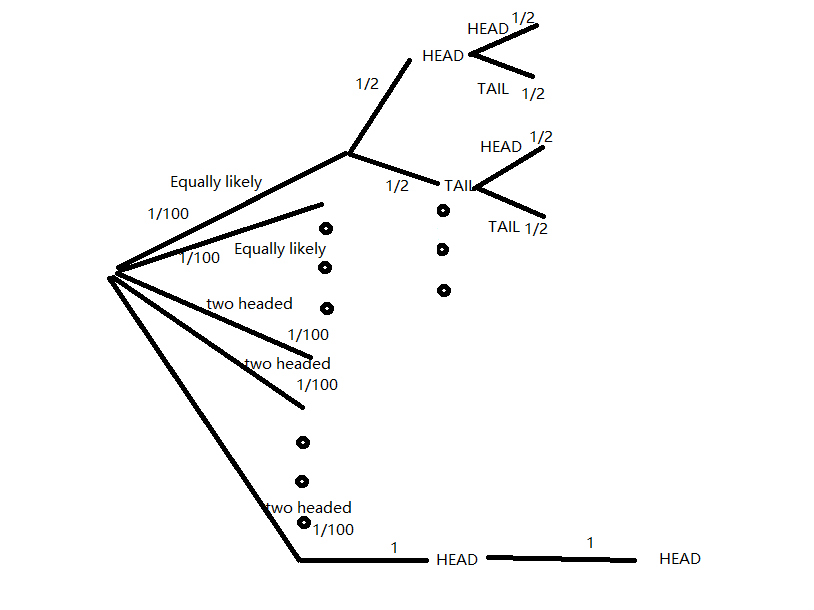
\includegraphics[scale = 0.3]{"C:/Users/Micha/OneDrive - Rensselaer Polytechnic Institute/CSCI 2200/Latex_pictures/PROB-TREE.png"}
	\end{figure}
	(a). According to the probabability tree, we have $P(\text{2 heads}) = \sum_{i=1}^{95} \dfrac{1}{400} + \sum_{i=96}^{100} \dfrac{1}{100} = \dfrac{95}{400}+\dfrac{5}{100} = \dfrac{23}{80}$.\\
	
	(b). According to the probabability tree, we have $P(\text{2 tails}) = \sum_{i=1}^{95} \dfrac{1}{400} + \sum_{i=96}^{100} 0 = \dfrac{95}{400} =  \dfrac{19}{80}$.\\
	
	(c). According to the probabability tree, we have $P(\text{2 tosses match}) = \sum_{i=1}^{95} \dfrac{2}{400} + \sum_{i=96}^{100} \dfrac{1}{100} = \dfrac{90}{400}+\dfrac{5}{100} = \dfrac{21}{40}$.
\end{addmargin}
%Q 11.71(a) ends here

\clearpage
%Q 12.31 starts from here
\begin{addmargin}[2em]{2em}
\text{\bf Problem 16.81.}You have a fair $5$-sided die which can generate one of the numbers $\{1, 2, 3, 4, 5\}$ with probability
$\dfrac{1}{5}$ each. You wish to simulate a fair $7$-sided die which generates a number in $\{1, 2, 3, 4, 5, 6, 7\}$ with probability $\dfrac{1}{7}$
each. Give an algorithm to do so, and prove it.\\

Toss a coint 2 twice, $\forall (i,j) \in \{1...5\}\times\{1...5\}$, we have $(1,1)=1,(2,2)=2,(3,3)=3,(4,4)=4,(5,5)=5,(5,1)=6,(5,2)=7$. Other wise, we restart.\\

Prove: Let $n$ be an arbitrary number and $n \in \{1,..,7\}$. We have 
\begin{align*}
	P[n]&=p[n|(1,1)]P[(1,1)]+p[n|(1,2)]P[(1,2)]+...+p[n|(i,j)]P[(i,j)]+P[n|restart]P[restart]\\
	P[n]&=\dfrac{1}{25}(\text{since there will be only 1 exact match}) + \dfrac{18}{25}P[n]\\
	\dfrac{17}{25}P[n]&=\dfrac{1}{25}\\
	P[n] &= \dfrac{1}{7}\\
\end{align*}
\end{addmargin}
%Q 12.31 ends here

\clearpage

%Q 12.74(k) starts from here
\begin{addmargin}[2em]{2em}
\text{\bf Problem 17.35}. You have 100 and bet 1 at a time on roulette. You goal is to win 50. Compute the probability that you reach your goal before going bankrupt.\\

I here assume it is exactly the same roulette as the one on the book.

probability of landing on red (probability of winning) = $\dfrac{18}{38}$. There are fifty steps away from winning, thus $L=150$.
The formula is $P(k,l,p) = \dfrac{p^k-p^l}{p^k-1}$.\\
Thus we have $P[win] = P(50,150,p) = \dfrac{0.9^{150}-0.9^{50}}{0.9^{150}-1} = 2.64 \times 10^-5$.
\end{addmargin}
%Q 12.74(k) ends here
\newpage
%Q 12.74(k) starts from here
\begin{addmargin}[2em]{2em}
	\text{\bf Problem 18.82}. You have N coins in your pocket. N is unknown and has a Poisson PDF, P[N = k] = $P[N = k] = \dfrac{e^{-2}2^k}{k!}$.
	You toss all the coins. What is the PDF for the number of H you get?\\
	
	$P[N = k] = \dfrac{e^{-2}2^k}{k!}$.
	Since the probability of getting head is one half, thus we have
	
	$P[\dfrac{N}{2} = k] = P[N=2k] = \dfrac{e^{-2}2^{2k}}{2k!}$.
\end{addmargin}
%Q 12.74(k) ends here
\end{document}